\documentclass{article}

% use Unicode characters - try changing the option if you run into troubles with special characters (e.g. umlauts)
\usepackage[utf8]{inputenc}

\usepackage{graphicx} % more modern
\usepackage{subcaption} 

% For citations
\usepackage{natbib}
\usepackage{url}

% For algorithms
\usepackage{algorithm}
\usepackage{algorithmic}
\usepackage{hyperref}
\usepackage{booktabs}
\usepackage{multirow}
\usepackage{amsmath}

\usepackage{array}

% \usepackage{dblfloatfix}
% \usepackage{fixltx2e}


\usepackage[accepted]{icml2017}

\def\docTitle{Inception U-Net: Ultrasound Nerve Segmentation}

\icmltitlerunning{\docTitle}
\title{Inception U-Net}

\begin{document} 

\twocolumn[
\icmltitle{\docTitle}

% It is OKAY to include author information, even for blind
% submissions: the style file will automatically remove it for you
% unless you've provided the [accepted] option to the icml2013
% package.

\begin{icmlauthorlist}
\icmlauthor{Peter James Bernante}{cs} \\
{\tt\small Maharishi University of Management} \\
{\tt\small pjbernante@mum.edu}
\end{icmlauthorlist}

\icmlaffiliation{cs}{Computer Science Department, Maharishi University of Management, Iowa, USA}

\icmlcorrespondingauthor{Peter James Bernante}{pjbernante@mum.edu}

% You may provide any keywords that you 
% find helpful for describing your paper; these are used to populate 
% the "keywords" metadata in the PDF but will not be shown in the document
\icmlkeywords{healthcare, medical imaging, convolutional neural networks, ultrasound, brachial plexus, nerve segmentation, segmentation}
\vskip 0.3in

\begin{abstract}
We develop an algorithm that can detect a collection of nerve structures called the Brachial Plexus (BP) \cite{wiki:Brachial_plexus}.
Our algorithm, Inception U-Net, is a deep convolutional neural network trained on ultrasound images from \cite{kaggle:ultrasound-nerve-segmentation}. The images were manually annotated by humans who were experts. We used a modified U-Net \cite{2015arXiv150504597R} architecture, and replaced its VGG-like \cite{2014arXiv1409.1556S} layers with Inception Modules \cite{2015arXiv151200567S}. We find that the Inception Modules made the model deeper and significantly reduced the number of parameters. We also found that, although the number of parameters is only a fraction of the standard U-Net, it had better performance in terms of defined metrics. Our algorithm was also able to annotate the images where the human annotators could not.
\end{abstract}
\bigskip
]
\printAffiliationsAndNotice{}

\section{Introduction}
Surgery oftentimes involves post-surgical pain. Managing pain involves the use of narcotics which have several unwanted side effects; under or overdosing respiratory side effects and sedation.

One way to manage pain with less dependency on narcotics is through the use of indwelling catheters that deliver anesthetic. Pain management catheters block or mitigate the pain at the source. These catheters are inserted in the area around the nerves that carries sensation from the surgical site. It is therefore imperative to accurately identify nerve structures in order to effectively insert the catheters.

The goal of this project is to identify a collection of nerve structures called the Brachial Plexus (BP) . Given an ultrasound image, highlight or annotate the area in the image where the BP is located.

We will apply deep learning in computer vision to recognize the BPs in ultrasound images. In doing so, the following tasks will be involved:
\begin{enumerate}
  \item Identify a collection of nerve structures called the Brachial Plexus.
  \item Given an ultrasound image, annotate the area in the image where BP is present
  \item Design a deep neural network to accomplish the task.
\end{enumerate}
The generated trained model can be useful in several ways. For example, it can be integrated with ultrasound apparatus to automatically show the area of interest.

\bigskip

\section{Problem Formulation}
The nerve identification task is a classification problem, where the input is an ultrasound image and the output is a binary label $t \in \{0,1\}$. We want to classify each pixel in an ultrasound image as to whether it belongs to the BP (positive class) or not (negative class).

For this binary classification project, it is important to classify all positive classes, and it is also important that all positively identified classes are correct. $F_1$ score , where both precision and recall are considered, would be appropriate as the metric of choice to measure the performance of our model. The general formula for an $F-measure$ in terms of Type I and Type II errors is given as:
$$F_\beta=\frac{ (1+\beta^2) \cdot P_{true} }{ (1+\beta^2) \cdot P_{true}  + \beta^2 \cdot N_{false} + P_{false} }$$

where:
\begin{align*}
P_{true} &= {True \ Positive} \\
N_{false} &= {False \ Negative} \\
P_{false} &= {False \ Positive} \\
\beta &= 1
\end{align*}
\bigskip

\begin{figure}[h]
    \centering
    \begin{subfigure}[b]{0.6\linewidth}
        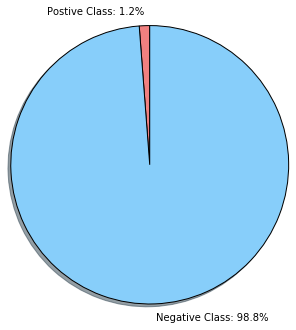
\includegraphics[width=1.0\linewidth]{figures/distribution_1.png}
        \caption{Classes are severely imbalanced}
        \label{fig:distribution_1}
    \end{subfigure}

   \begin{subfigure}[b]{0.7\linewidth}
        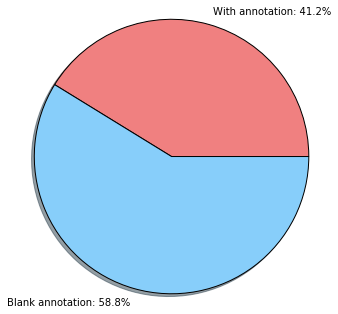
\includegraphics[width=1.0\linewidth]{figures/distribution_2.png}
        \caption{Majority of the images has blank annotations (i.e. no annotated brachial plexus)}
        \label{fig:distribution_2}
    \end{subfigure}

    \caption{Distribution of classes}
    \label{fig:distribution}
\end{figure}

\begin{figure}[h]
 \centering
  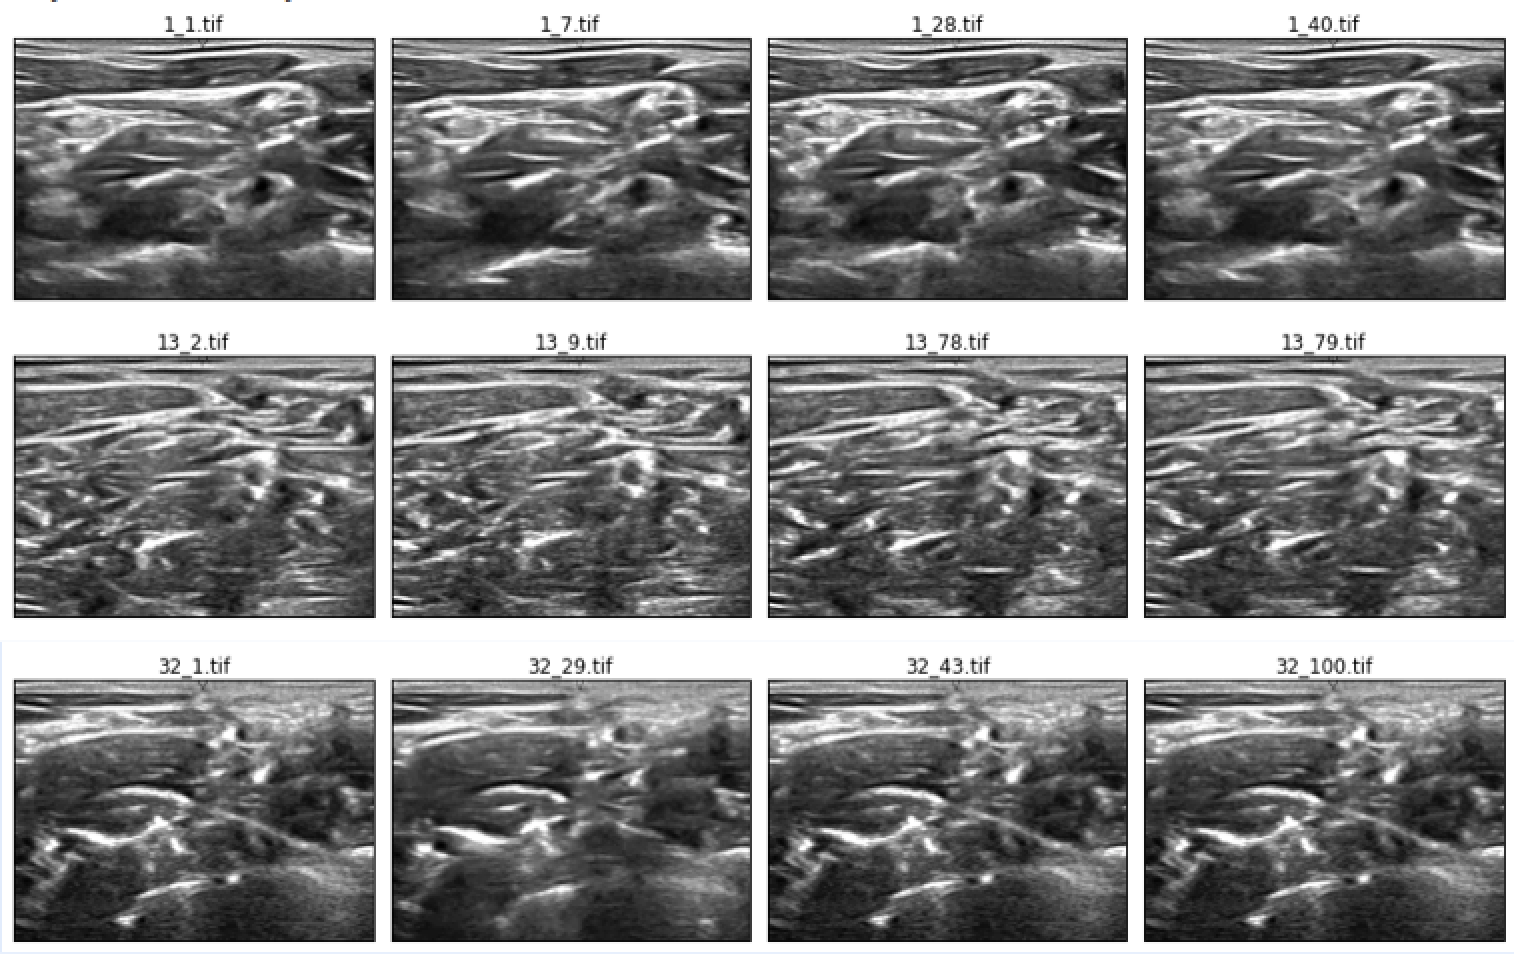
\includegraphics[width=1.0\linewidth]{figures/high_corr.png}
  \caption{
      High correlation of images. The file names have the format \textless patient\_id\_xxx.tif\textgreater . Images coming from the same patient ID are highly correlated. (NOTE: The images are not exactly the same.)
  }
  \label{fig:high_corr}
\end{figure}

\begin{figure}[h]
 \centering
  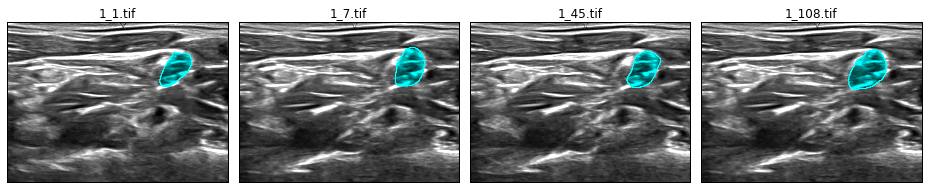
\includegraphics[width=1.0\linewidth]{figures/inaccurate_1.png}
  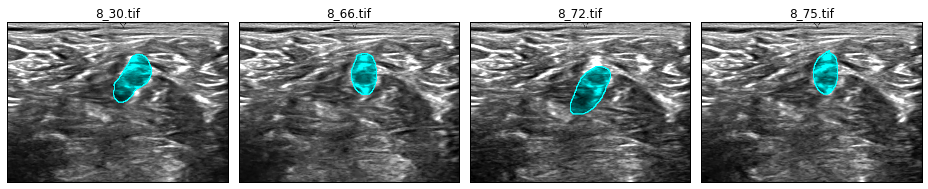
\includegraphics[width=1.0\linewidth]{figures/inaccurate_2.png}
  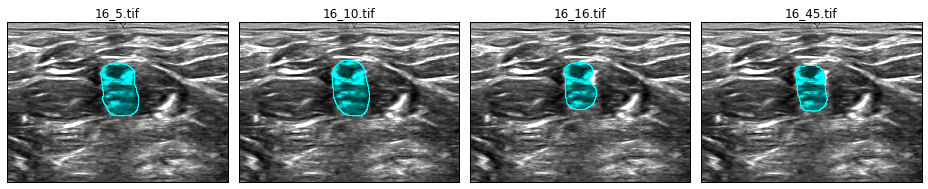
\includegraphics[width=1.0\linewidth]{figures/inaccurate_3.png}
  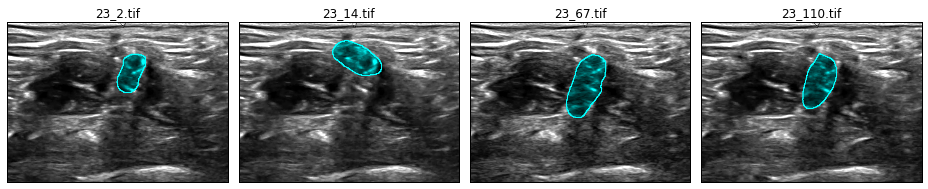
\includegraphics[width=1.0\linewidth]{figures/inaccurate_4.png}
  \caption{
      Similar images with varying annotations. Human-annotated training images have inaccurate annotations.
  }
  \label{fig:inaccurate}
\end{figure}


\begin{figure}[h]
 \centering
  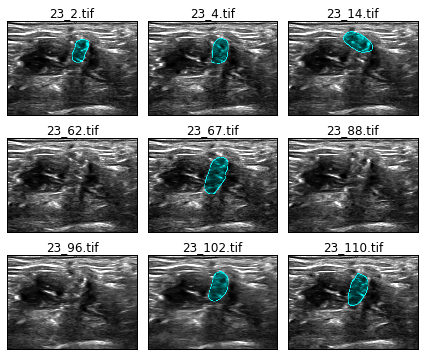
\includegraphics[width=1.0\linewidth]{figures/conflicting.png}
  \caption{
      Conflicting annotations. Very similar images have conflicting annotations. One image has BP while the other has none. These are human errors during manual annotation of the dataset.
  }
  \label{fig:conflicting}
\end{figure}


\begin{figure}[h]
 \centering
  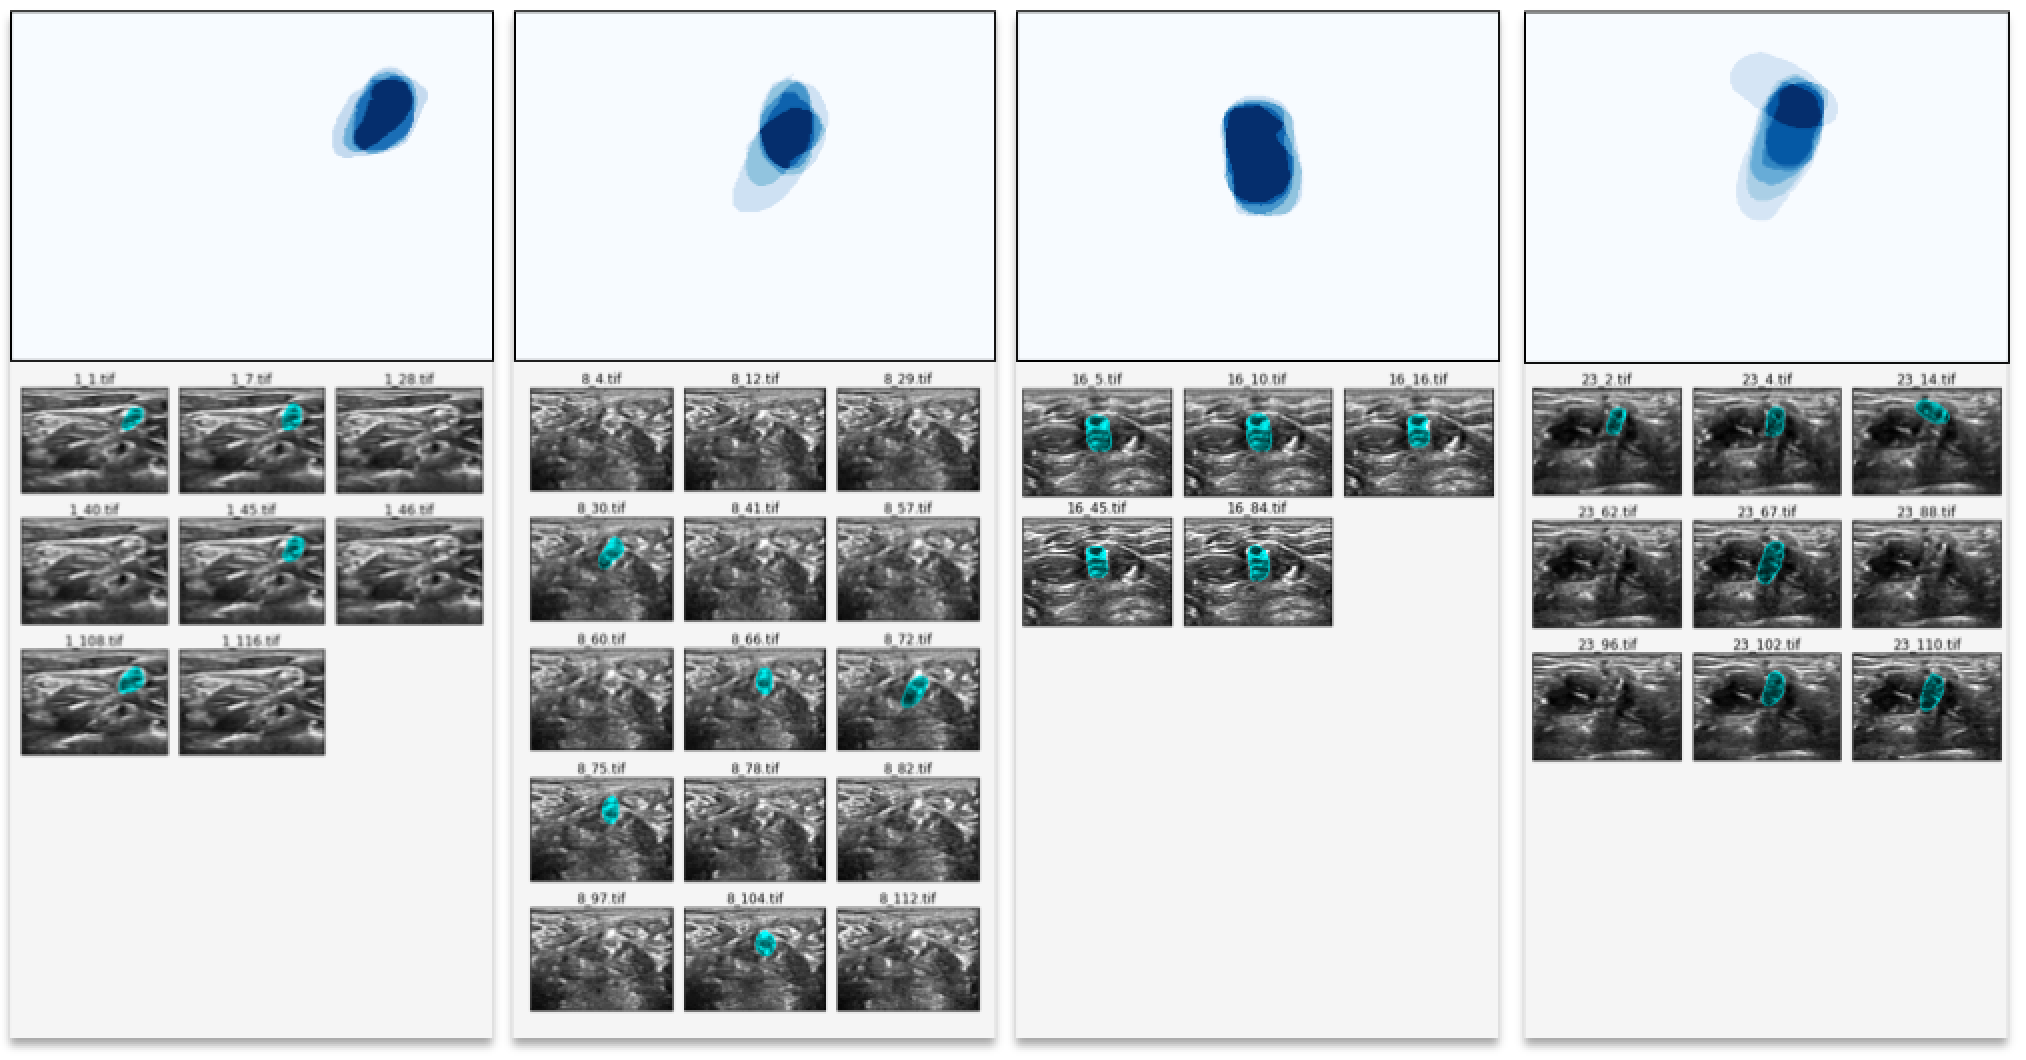
\includegraphics[width=1.0\linewidth]{figures/average_loc.png}
  \caption{
      Average annotations of similar images. Similar images have similar annotations, if present. The annotations do not exactly have the same shape, but they cover the same general area of the image and have common intersections.
  }
  \label{fig:average_loc}
\end{figure}

\begin{figure*}[ht]
 \centering
  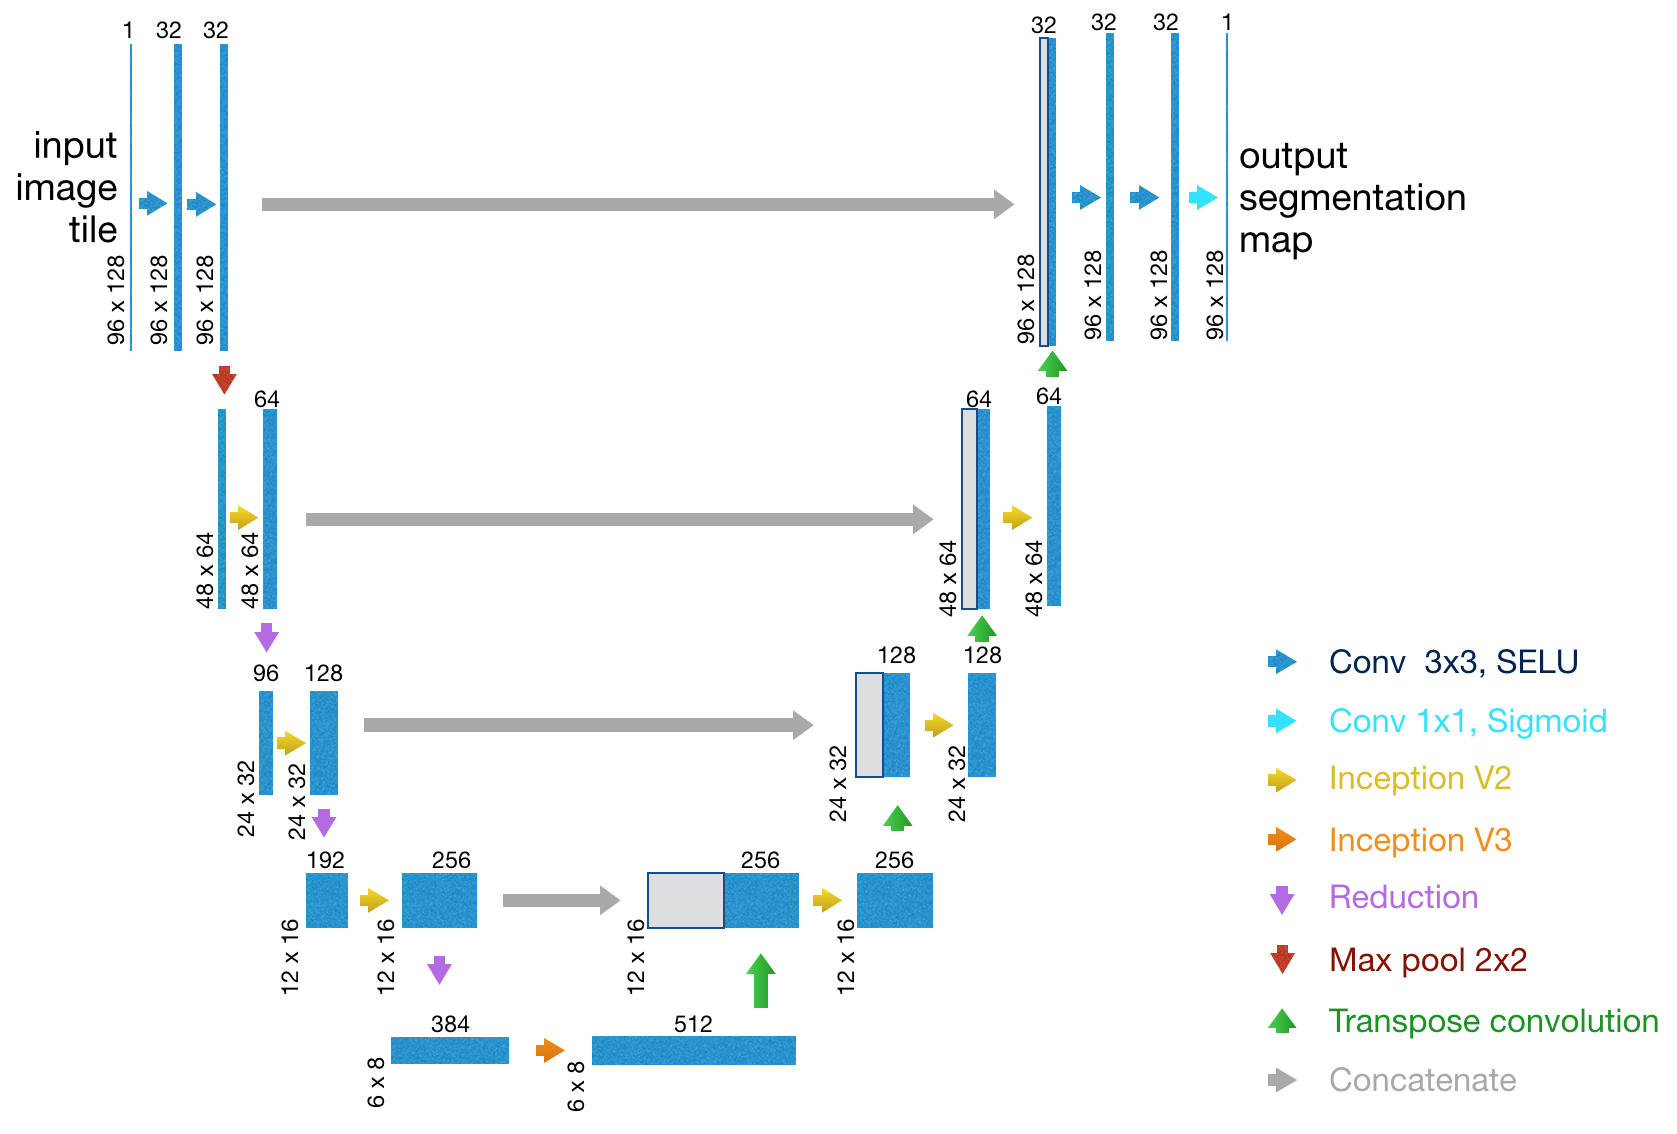
\includegraphics[width=0.8\linewidth]{figures/inception-u-net.png}
  \caption{
      Inception U-Net Architecture. All layers in the middle uses Inception V3 and Grid Reduction modules instead of VGG and MaxPooling. Inception V4 is used in the coarsest layer at the bottom. Transpose Convolution is used to upsample the layer to the same size as the input. All Layers used SELU activation, with the exception of the last layer where Sigmoid was used for binary classification.
  }
  \label{fig:inception-u-net}
\end{figure*}




\section{Data Exploration}
There are 5,635 images for training and 5,508 images for testing. The images are gray scale with dimensions 580 x 420 pixels and are noisy. Training images have masks to indicate where the BP is present, while there is none for testing images. In the training images, only 2,323 images have positively identified the BP.
Groups of images are taken from the same patient.  Images that come from the same patient are highly correlated (see Figure \ref{fig:high_corr}).

The classes are severely imbalanced; consisting of $1.2\%$ positive class and $98.8\%$ negative class (see Figure \ref{fig:distribution}. This class imbalance is mitigated by using $F_1$ score.

There are inaccuracies in the annotations of the BP. There is no prefect ground truth or gold standard (see Figure \ref{fig:inaccurate}). There are very similar images but with conflicting annotations; one image has positively identified the BP, however the other has none (see Figure \ref{fig:conflicting}). There are also very similar images that have positive annotations, but the area where they are annotated differ in shape/area, although the annotations are located approximately in the same region (see Figure \ref{fig:average_loc}).

Where the BP is present in an image, the BP annotations has the following characteristics:

\begin{center}
\begin{tabular}{l r}
Minimum size &    2,684 pixels \\
Maximum size &   17,439 pixels \\
Average size & 7,125.74 pixels \\
\end{tabular}
\end{center}

\bigskip

\section{Data Preprocessing}

\subsection{Filtering}
As shown in Figure \ref{fig:conflicting}, several images are very similar but have conflicting masks. This will greatly negatively affect the learning process. To mitigate the negative impact, images without masks, but with very similar images that have masks, are filtered out (images without masks and have no similar images are retained). The reason for dropping these images is, they most likely have similar annotation with their annotated counterpart, and were overlooked during manual annotations (it is more likely to miss to annotate an image than accidentally annotating random location of the image).

For similar images with varying annotations (in terms of shapes and sizes), they mostly cover the same general area of the image, and have common intersections. These images are retained for training to force the model to figure out what is common between the annotations.

The similarity of the images are measured using normalized cross-correlation coefficient \cite{cross-correlation} with a threshold of 0.8.


\subsection{Resizing Images}
The ultrasound images are large files and have a lot of noise. To reduce the noise, the images are downsized to 96 x 128 pixels using inter-area interpolation \cite{GEAN:GEAN1135}. Downsizing also significantly reduces the dimensionality of the dataset, which will also improve the training time.

\subsection{Splitting}
The dataset is split to 80\% train and 20\% validation sets. The split is stratified based on the presence of mask.

\subsection{Normalization}
To have better training performance, the dataset is centered at zero mean and normalized to unit variance. This was done by subtracting the mean and then dividing by the standard deviation of the dataset.
\bigskip


\section{Model Architecture}
In this semantic image segmentation problem, a deep neural network will be used to predict the labels for each pixel in the image. Convolutional networks \cite{Lecun98gradient-basedlearning}, from which most state of the art image recognition techniques are derived, will used as the building block of our architecture.

In our dataset, the pixels are roughly similar all throughout the image. There is no clear groupings or sharp boundaries in which an untrained eye can clearly identify the brachial plexus.

The U-Net architecture \cite{2015arXiv150504597R} uses VGG-like layers \cite{2014arXiv1409.1556S}, where a series of convolutional layers are place on top of each other, and gradually decreasing the grid size while increasing the depth. The convolutions are then gradually reversed until the layer is back to its original size. This forms a U-like structure, from which the architecture got its name.

Marko Jocic \cite{jocicmarko-ultrasound-segmentation} has demonstrated the use of U-Net on the same dataset. Our architecture improves U-Net by replacing the VGG-like layers with Inception Modules \cite{2015arXiv151200567S} (See Figure \ref{fig:inception-u-net}). All layers in the middle uses Inception V3 and Grid Reduction modules instead of VGG and MaxPooling. Inception V4 is used in the coarsest layer at the bottom. Transpose Convolution \cite{2016arXiv160307285D} is used to upsample the layer to the same size as the input. The Inception modules made the model so deep and results to vanishing gradients. To solve this, SELU \cite{2017arXiv170602515K} activations are used which make it impossible to have vanishing or exploding gradients. Sigmoid was used at the last layer for binary classification (see Table \ref{tab:comparison}).
\begin{table}[h]
	\centering
	\begin{tabular}{l c c}
	\toprule
	\ & U-Net & Inception U-Net \\
	\midrule
	\midrule
 	Parameters & 7,759,521\footnotemark  & 1,846,353\footnotemark[\value{footnote}] \\
	File size       & 93 MB\footnotemark[\value{footnote}]       & 22.7 MB\footnotemark[\value{footnote}] \\
    Layer           & VGG-like    & Inception Module \\
	Pooling			& Max pooling & Reduction Module \\
    Activations     & ReLU        & SELU \\
	\bottomrule
		
	\end{tabular}
	\caption{Comparison of U-Net and Inception U-Net.}
\label{tab:comparison}
\end{table}

\footnotetext{Based on 96 x 128 input shape}
\bigskip

\begin{figure}[h]
 \centering
  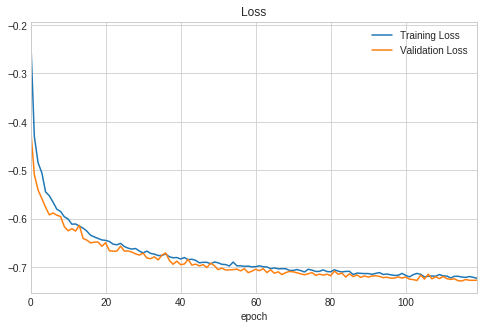
\includegraphics[width=1.0\linewidth]{figures/loss.png}
  \caption{
      Training and Validation Loss
  }
  \label{fig:loss}
\end{figure}

\begin{figure}[h]
 \centering
  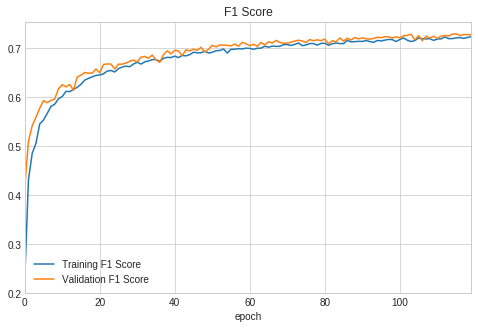
\includegraphics[width=1.0\linewidth]{figures/f1.png}
  \caption{
      Training and Validation $F_1$ Scores
  }
  \label{fig:f1}
\end{figure}

\section{Training}
\subsection{Loss Function}
We want our output to produce similar mask as the labels. This entails a measure of similarity. Dice Coefficient \cite{Sorensen-1948-BK} is a static used for comparing the similarity of two samples, and is given with the formula:

$$QS=\frac{2|X\bigcap Y|}{|X| + |Y|}$$

It was originally intended to be applied to presence/absence of data. ${QS}$ is the quotient of similarity and ranges between 0 and 1, where 1.0 means the two samples are exactly the same. It can be viewed as a similarity measure over sets.

The loss function minimizes, so we take the negative Dice Coefficient as our loss function.

\subsection{Training Configuration}
Training the model was run with the following configuration:

\begin{center}
\begin{tabular}{r l}
	Optimizer           & Adam \\
	Learning rate       & 0.0001 \\
	Learning rate decay & 0.001 \\
	Loss Function       & - Dice Coefficient \\
	Batch size          & 32 \\
	Epochs              & 120
\end{tabular}
\end{center}

The weights of the network were randomly initialized and trained end-to-end using Adam optimizer \cite{2014arXiv1412.6980K} default values for hyperparameters $\beta_1=0.9$ and $\beta_2=0.999$. The learning rate was set to 0.0001 with a decay of 0.001 for every iteration.

With limited training dataset, data augmentation was applied. Artificial images were generated on-the-fly which consists of transformation of the images including horizontal and vertical shifts, rotation between $\pm30$ degrees, up to 10\% zoom, and horizontal and vertical flips.

We use Keras \cite{chollet2015keras} to run the training with TesnsorFlow \cite{tensorflow2015-whitepaper} backend.


\subsection{Evaluation and Validation}
The learning rate that produced reasonable result is around 0.0001. Higher learning rate converged to higher loss value while with lower learning the training was not able to converge after several epochs. Exponential learning rate decay of 0.001, decayed at every iteration, helped stabilized the loss convergence at the later stage of training.

The training and validation loss were very close to each either which indicates that the model is neither overfitting nor has high variance (See Figure \ref{fig:loss}).

The $F_1$ score also shows a result that is in agreement with the loss (See Figure \ref{fig:f1}).

The final model was chosen using early stopping. The checkpoint with highest validation score was chosen as the final model. The validation set uses images that were not included during training. It generally has lower score compared to training, which reflects more accurate performance metric of the model.


To verify the robustness of the model, inference was run using the test dataset. This dataset does not have accompanying ground truth that can be compared with to produce a quantitative measure. It is rather difficult for untrained eyes to make a judgment as to whether or not the predicted annotations are accurate. As a non-medical professional, we can look over and again the training set and pick up general pattern of nerve structures. However, this would still be not very reliable and consulting with a trained medical professional would be best to verify the result. Some samples predictions using the test dataset are shown in Figure \ref{fig:result_3} for qualitative assessment.
\bigskip


\begin{figure*}[ht]
    \centering
    \begin{subfigure}[b]{1.0\linewidth}
        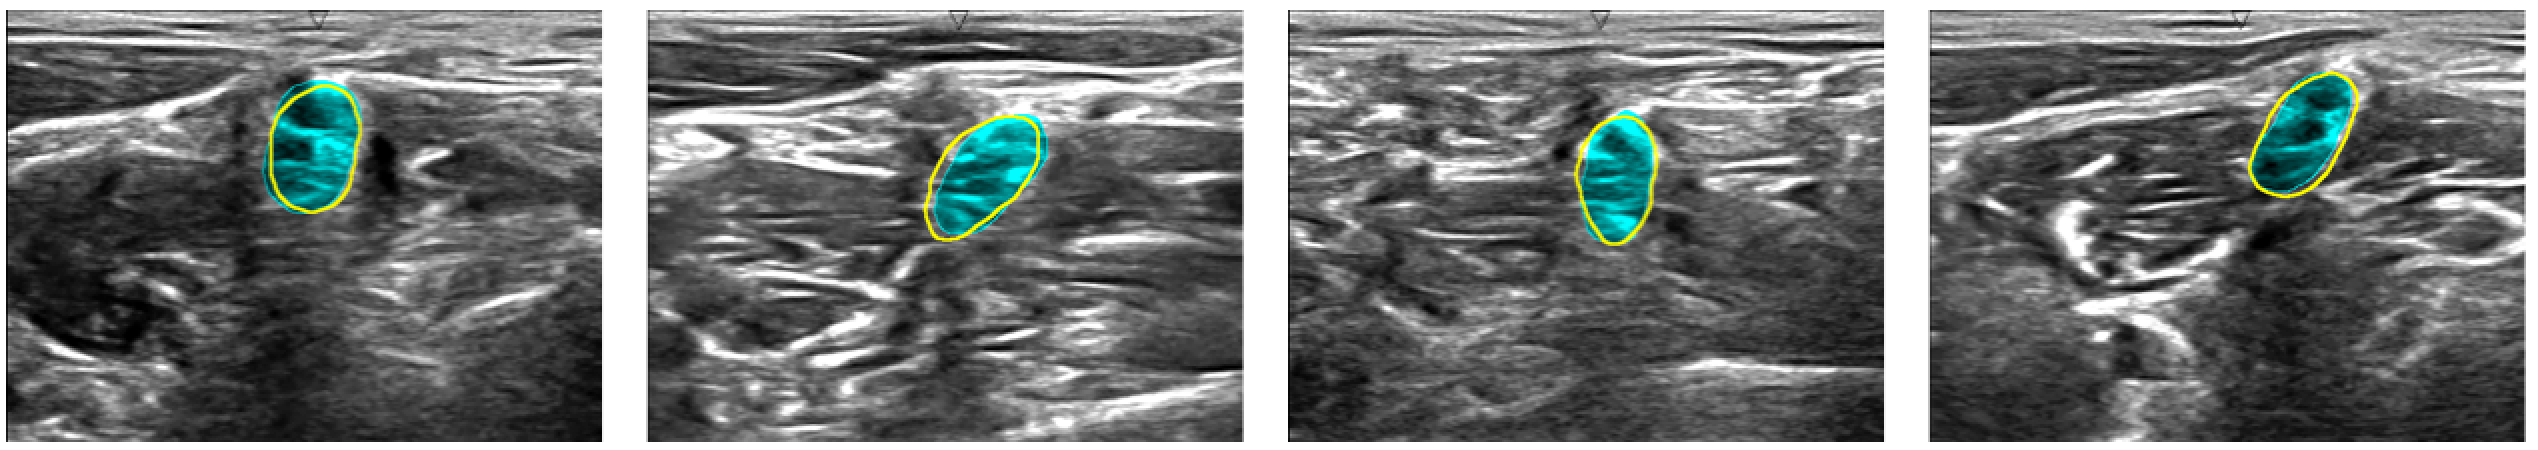
\includegraphics[width=1.0\linewidth]{figures/result_1.png}
        \caption{Good performance of the model. The area highlighted in cyan is the ground truth while the area outlined in yellow is the prediction of the model. The model predictions are almost identical to the ground truth.}
        \label{fig:result_1}
    \end{subfigure}
    
    \begin{subfigure}[b]{1.0\linewidth}
        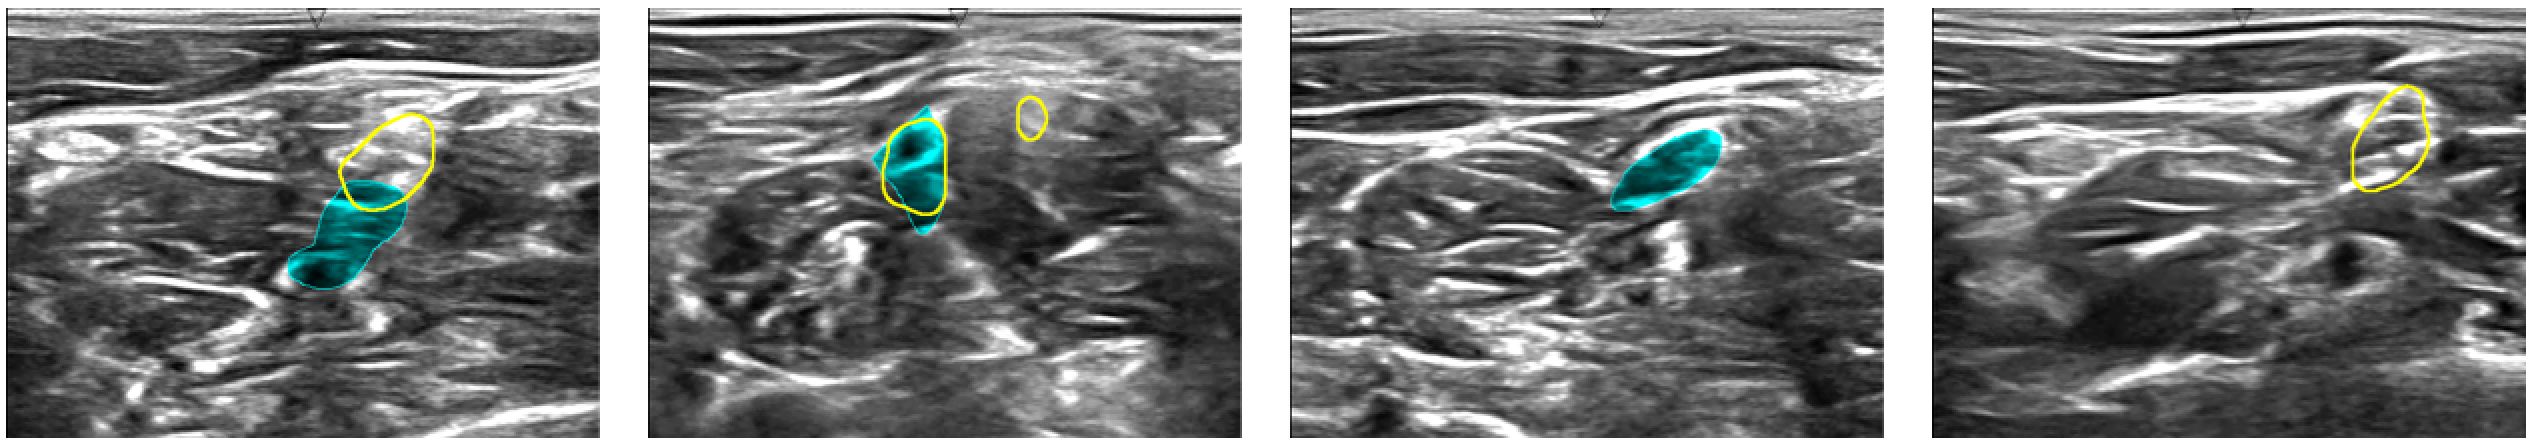
\includegraphics[width=1.0\linewidth]{figures/result_2.png}
        \caption{Missed out predictions. From left to right: (a) the model prediction mostly missed the ground truth, (b) the model hit the ground truth but also annotated an extra area, (c) the model was not able to detect brachial plexus but there actually exists, and (d) the model was able to find brachial plexus where human annotator missed out.}
        \label{fig:result_2}
    \end{subfigure}
    
    \begin{subfigure}[b]{1.0\linewidth}
        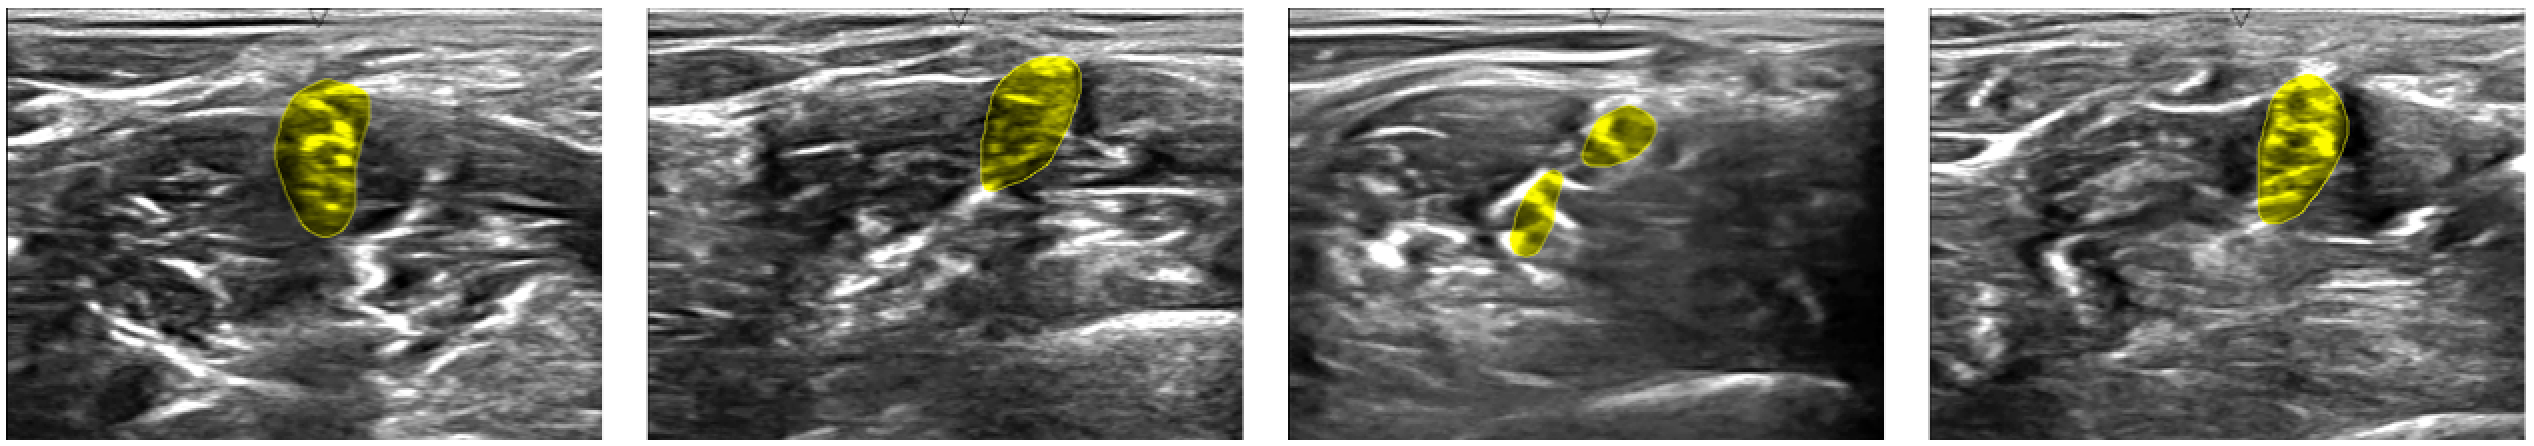
\includegraphics[width=1.0\linewidth]{figures/result_3.png}
        \caption{Inference on test dataset. The yellow highlights are the prediction of the model. The test dataset has no accompanying ground truth to compare the results with. Consultation from trained ultrasound professional is needed.}
        \label{fig:result_3}
    \end{subfigure}


    \caption{Final Model Output}
    \label{fig:result}
\end{figure*}

\section{Result}

Some images from validation and test set that were not used in training were evaluated. It can be seen that the model performs well on most images. However, there are also cases where it misses. The area highlighted in cyan is the ground truth while the area outlined in yellow is the prediction produced by the model (See Figure \ref{fig:result}). 
\bigskip




\bibliographystyle{icml2017}
\bibliography{main}


\end{document} 

